%-------------------------------------------------------------------------------
%	PORTADA
%-------------------------------------------------------------------------------

$if(has-frontmatter)$
\frontmatter
$endif$

$if(title)$
\cleardoublepage

\thispagestyle{empty}

{\centering


\includegraphics{assets/escudo_udea.png}

\vspace{2cm}
{\bfseries $title$}\\[2cm]

\vspace{2cm}
$for(by-author)$
{$by-author.name.literal$}\\
$endfor$

\vspace{2cm}
{$tipo-documento$ para optar al título de $titulo-otorgado$}

\vspace{2cm}
{$tipo-orientador$}\\
{$nombre-orientador$, $titulo_orientador$}

\vspace{1cm}
{Universidad de Antioquia}\\
{$unidad-academica$}\\
{$programa$}\\
{$ciudad$}\\
{$ano-grado$}

}
$endif$
\newpage

%-------------------------------------------------------------------------------
%	CITACIÓN
%-------------------------------------------------------------------------------

\thispagestyle{empty}
\begin{center}
\begin{table}
  \arrayrulecolor{verdeUdeA}
  \footnotesize
  \begin{tabular}{cm{10cm}} 
    \noalign{\color{verdeUdeA}\hrule height 3pt}
    \textbf{Cita} & \hspace{2cm}($citacion$, $ano-grado$) \\
    \hline
    \textbf{\parbox[c][1.6\height]{5cm}{\centerline{Referencia} 
        \vspace*{0.5cm}\centerline{Estilo APA 7 (2020)}}}
    & \hspace{-0.5cm}$referencia$ ($ano-grado$). \textit{$title$} [$modalidad-grado$]. Universidad de Antioquia, $ciudad$. \\ 
    \noalign{\color{verdeUdeA}\hrule height 3pt}
  \end{tabular}
  \arrayrulecolor{black}
\end{table}
\end{center}
%
$if(licencia-tipo)$
\vspace{-2.3cm}
\noindent
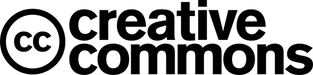
\includegraphics{assets/license/cc-logo.png}\quad
\includegraphics{$licencia-tipo$}
$endif$

\vspace{1cm}
$if(cohorte-posgrado)$
\noindent
{$programa$, Cohorte $cohorte-posgrado$}\\
{Grupo de Investigación $grupo-investigacion$}\\
{$centro_investigacion$}\\[1cm]
$endif$
%

\includegraphics{assets/escudo_udea_vice.png}\quad

\includegraphics{assets/sis_biblo.png}\\
{$biblioteca$}\\[1cm]
%
{\textbf{Repositorio Institucional:} \url{http://bibliotecadigital.udea.edu.co}}\\[1cm]
{Universidad de Antioquia - \url{www.udea.edu.co}}\\[0.5cm]
%
{\textbf{Rector:} $rector$}\\
{\textbf{Decano/Director:} $decano-director$}\\
{\textbf{Jefe departamento:} $jefe-departamento$}\\[1cm]
%
El contenido de esta obra corresponde al derecho de expresión de los autores y no compromete el pensamiento institucional de la Universidad de Antioquia ni desata su responsabilidad frente a terceros. Los autores asumen la responsabilidad por los derechos de autor y conexos.
\newpage

%-------------------------------------------------------------------------------
%	CITA
%-------------------------------------------------------------------------------

$if(cita)$

\thispagestyle{empty}

\vspace*{0.2\textheight}

$if(cita.texto)$
\noindent``{\itshape $cita.texto$}''\bigbreak

\hfill {$cita.autor$}
$else$
\input{``$cita$''}
$endif$

$endif$
\newpage

%---------------------------------------------------------------------------------------
%	DEDICATORIA
%---------------------------------------------------------------------------------------

$if(dedicatoria)$

\thispagestyle{empty}

\vspace*{0.3\textheight}

{$dedicatoria$}

$else$
\input{"$dedicatoria$"}

$endif$
\newpage

%-------------------------------------------------------------------------------
%	AGRADECIMIENTOS
%-------------------------------------------------------------------------------


$if(agradecimientos)$
\thispagestyle{empty}

\addchap*{Agradecimientos}

$agradecimientos$

$else$
\input{"$agradecimientos$"}

$endif$
\newpage

%-------------------------------------------------------------------------------
%	TOC, LOT, and LOF
%-------------------------------------------------------------------------------

\begingroup
$if(toc-title)$
\renewcommand*\contentsname{$toc-title$}
$endif$
$if(colorlinks)$
\hypersetup{linkcolor=$if(toccolor)$$toccolor$$else$$endif$}
$endif$
$if(toc-depth)$
\setcounter{tocdepth}{$toc-depth$}
$endif$
$if(toc)$
\tableofcontents
$endif$
$if(lot)$
\listoftables
$endif$
$if(lof)$
\listoffigures
$endif$
\endgroup